\section{Modulationsarten}
Modulationsverfahren sind ein großes Anwendungsgebiet in der Nachrichtentechnik.
Ziel ist es viele Informationen Verlustfrei zu übertragen.
Möchte man ein Datensignal übertragen muss es davor
aufbereitet werden. Dies erledigt der Modulator/Mischer.
\\
Es gibt Analoge und Digitale Modulationsarten.
Für Analoge Signale werden folgende Verfahren verwendet.


\subsection{Amplitudenmodulation AM}
Die Idee hinter der Amplitudenmodulation ist dass das Informationssignal
auf die Amplitude des Trägersignals zu modulieren.
Daduch veränder sich die Amplituder des Trägersignals in abhängigkeit des Pegels und 
Freqeuenz des Informationssignals.
\\
\begin{figure}[h]
    \centering
    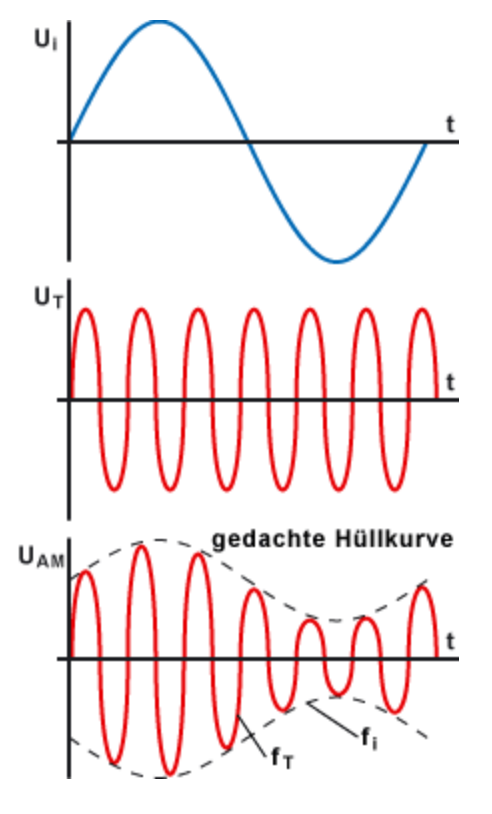
\includegraphics[width=0.22\textwidth]{Pictures/Screenshot 2025-06-19 125508.png}
    \caption{Amplitudenmodulation}
    \footnotesize{Quelle: \url{https://www.elektronik-kompendium.de/sites/kom/0401181.htm}}
    \label{fig:link_budget}
\end{figure}
\clearpage
Die Amplitude der Trägerschwingung wird durch das analoge Datensignal
$x(t)$ folgendermaßen verändert.
\begin{equation}
    a(t)=A_c(1+\mu x(t))
\end{equation}
Das AM-Signal wird beschrieben durch.
\begin{equation}
    x_c(t)=A_c(1+\mu x(t))cos(2\pi f_c t)
\end{equation}
\begin{itemize}
    \item $A_c$: Trägeramplitude
    \item $f_c$: Trägerfrequenz
    \item $\mu$: Modulationsindex 0 < $\mu$ < 1
\end{itemize}


\subsection{Frequenzmodulation FM}
Die Frequenzmodulation spielt eine eben so wichtige Rolle wie die Amplitudenmodulation,
ist im vergleich jedoch weniger Störanfällig. 
Hier wird auch ein hochfrequentes Trägersignal erzeugt und dadurch die Sendefrequenz um ein kleinen Betrag verändert.
Am einfachsten ist so eine Modulation durch ein LC-Schwingkreis.

\begin{equation}
x_c(t) = A_c \cos\left( 2\pi f_c t + 2\pi f_\Delta \int_0^t x(\tau) \, \mathrm{d}\tau \right)
\end{equation}
\begin{itemize}
    \item $x(\tau)$: Datensignal
    \item $A_c$: Amplitude des Trägersignals (konstant)
    \item $f_c$: Trägerfrequenz 
    \item $f_\Delta$: Frequenzhub, legt die maximale abwichung zu $f_c$ fest
\end{itemize}
\clearpage

\subsection{Phasenmodulation PM}
Die Phasenmodulation gehört wie die Frequenzmodulation zu den Winkelmodulationen.
Hier wird die Phase der Trägerwelle in Abhängigkeit des Datensignals verändert.
Die Phasenveränder bleibt im Signal erhalten variiert jedoch im vergleich
zur Ursprünglichen Phase des Trägersignal
\begin{figure}[h]
    \centering
    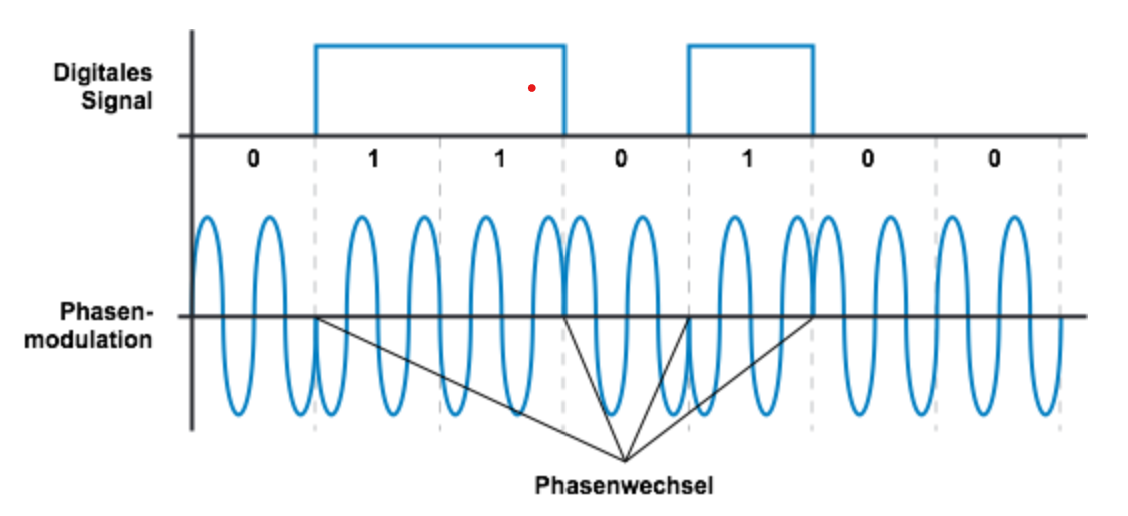
\includegraphics[width=0.5\textwidth]{Pictures/04020211.png}
    \caption{Phasenmodulation}
    \footnotesize{Quelle: \url{https://www.elektronik-kompendium.de/sites/kom/0402021.htm}}
\end{figure}

\section{Blockdiagramm einer Sendestrecke}
\subsection{DAC}
\subsection{LO}
\subsection{Mischer} 
\subsection{PA}
\subsection{Antennen}
\subsection{LNA}
\subsection{Demodulation}
\subsection{ADC}


\section{Mathematische Grundlagen: Fourier-Transformation}
\subsection{Betrag und zeitlicher Verlauf von Rechteckfunktion}
\subsection{Betrag und zeitlicher Verlauf von Sinusfunktion}
\subsection{Multiplikation der beiden Funktionen im Zeitbereich}


\section{Zusammenhang von Datenrate und Bandbreite}
blabla
\clearpage